\documentclass[aspectratio=169,11pt]{beamer}

\usepackage[utf8]{inputenc}
\usepackage[T1]{fontenc}
\usepackage[brazil]{babel}
\usepackage[sfdefault,light]{FiraSans}
\usepackage{booktabs}
\usepackage{array}
\usepackage{graphicx}
\usepackage{listings}
\usepackage{tikz}
\usepackage{pgfplots}
\usepackage{xcolor}
\usepackage{hyperref}
\usetikzlibrary{arrows.meta,calc,positioning,shapes.geometric}
\pgfplotsset{compat=1.18}

\definecolor{caipyraWine}{HTML}{963435}
\definecolor{caipyraRed}{HTML}{D11E00}
\definecolor{caipyraOrange}{HTML}{FC7E00}
\definecolor{caipyraYellow}{HTML}{FFFD98}
\definecolor{caipyraInk}{HTML}{364153}
\definecolor{caipyraMuted}{HTML}{6B7280}
\definecolor{caipyraPaper}{HTML}{F9FAFB}
\definecolor{caipyraNavy}{HTML}{101828}
\definecolor{caipyraLine}{HTML}{E5E7EB}

\mode<presentation>{
  \usetheme{default}
  \usecolortheme{default}
  \setbeamertemplate{navigation symbols}{}
  \setbeamertemplate{footline}{}
  \setbeamertemplate{headline}{}
}

\setbeamercolor{normal text}{fg=caipyraInk,bg=white}
\setbeamercolor{frametitle}{fg=caipyraRed,bg=white}
\setbeamercolor{title}{fg=white,bg=caipyraRed}
\setbeamercolor{subtitle}{fg=white,bg=caipyraRed}
\setbeamercolor{block title}{fg=white,bg=caipyraRed}
\setbeamercolor{block body}{fg=caipyraInk,bg=caipyraPaper}
\setbeamerfont{frametitle}{series=\bfseries,size=\Large}
\setbeamerfont{title}{series=\bfseries,size=\huge}
\setbeamerfont{subtitle}{size=\large}
\setbeamerfont{block title}{series=\bfseries}
\setbeamertemplate{itemize item}{\color{caipyraRed}\raisebox{0.18ex}{\scriptsize$\blacktriangleright$}}
\setbeamertemplate{itemize subitem}{\color{caipyraOrange}\raisebox{0.18ex}{\tiny$\blacktriangleright$}}
\setlength{\parskip}{0.25em}

\hypersetup{
  colorlinks=true,
  urlcolor=caipyraRed,
  linkcolor=caipyraRed
}

\lstdefinestyle{py}{
  language=Python,
  basicstyle=\ttfamily\scriptsize,
  keywordstyle=\color{caipyraRed}\bfseries,
  commentstyle=\color{caipyraMuted},
  stringstyle=\color{caipyraWine},
  showstringspaces=false,
  columns=fullflexible,
  keepspaces=true,
  frame=single,
  framerule=0.35pt,
  rulecolor=\color{caipyraLine},
  backgroundcolor=\color{caipyraPaper},
  xleftmargin=0.4em,
  xrightmargin=0.4em,
  aboveskip=0.4em,
  belowskip=0.2em
}

\newcommand{\eyebrow}[1]{{\color{caipyraOrange}\small\bfseries #1}\par\vspace{0.25em}}
\newcommand{\callout}[1]{%
  \begin{beamercolorbox}[wd=\linewidth,sep=0.7em,rounded=true]{block body}
    #1
  \end{beamercolorbox}
}
\newcommand{\metric}[3]{%
  \begin{minipage}[t]{\linewidth}
    {\color{caipyraRed}\bfseries\Large #1}\par
    {\small\bfseries #2}\par
    {\footnotesize\color{caipyraMuted} #3}
  \end{minipage}
}
\newenvironment{tightitemize}{%
  \begin{itemize}\setlength{\itemsep}{0.25em}\setlength{\parskip}{0pt}
}{\end{itemize}}

\title{9 anos de ensino de Redes com Python}
\subtitle{onde dá conta de tudo, e onde foi preciso buscar alternativas}
\author{Prof. Paulo Matias (UFSCar)}
\date{sábado, 6 de junho de 2026, 14:50}

\begin{document}

{
\setbeamercolor{background canvas}{bg=caipyraRed}
\begin{frame}[plain]
  \vspace{1.2cm}
  {\color{white}\bfseries\fontsize{30}{34}\selectfont 9 anos de ensino de Redes com Python}\par
  \vspace{0.4cm}
  {\color{caipyraYellow}\Large onde dá conta de tudo, e onde foi preciso buscar alternativas}\par
  \vfill
  {\color{white}Prof. Paulo Matias (UFSCar) \hfill sábado, 6 de junho, 14:50}\par
  \vspace{0.25em}
  {\color{white}Caipyra 2026 -- Palestras -- Auditório Fernão \hfill Iniciante}
\end{frame}
}

\begin{frame}{Resumo da palestra}
  \begin{tightitemize}
    \item o recorte de 9 anos é Redes de Computadores com Python desde 2018
    \item a pilha implementada passa por IRC, TCP, IPv4, SLIP e hardware real em FPGA
    \item desde 2022, leciono Tecnologia de Comunicação, que é disciplina correlata
    \item nesse contraste, Python funciona bem em simulação e processamento offline
    \item no modem V.21, tempo real levou à migração para C++ e Rust
  \end{tightitemize}

  \vspace{0.8em}
  \callout{
    A pergunta da palestra é menos ``Python serve?'' e mais ``em que papel
    Python serve melhor?''.
  }
\end{frame}

\begin{frame}{Tese}
  \eyebrow{Ensino de Redes}
  \Large
  Python funciona bem quando a disciplina quer que estudantes implementem protocolos,
  não apenas configurem equipamentos ou o sistema operacional.

  \vspace{0.8em}
  \normalsize
  \callout{
    A aposta não foi ``Python é mais fácil''. A aposta foi: a linguagem deixa a
    pilha de protocolos suficientemente visível para testar, depurar e integrar
    em ambiente real dentro de um semestre.
  }
\end{frame}

\begin{frame}{O contraste que motivou a disciplina}
  \begin{columns}[T,onlytextwidth]
    \column{0.47\linewidth}
    \eyebrow{Ênfase comum}
    \begin{tightitemize}
      \item configurar roteadores, switches e serviços
      \item usar ferramentas do sistema operacional
      \item diagnosticar redes já prontas
      \item entender protocolos pelo comportamento externo
    \end{tightitemize}

    \column{0.47\linewidth}
    \eyebrow{Ênfase na UFSCar}
    \begin{tightitemize}
      \item implementar camadas da pilha
      \item construir contratos entre camadas
      \item passar de testes locais para cenário físico
      \item entender protocolos pelo estado interno
    \end{tightitemize}
  \end{columns}
\end{frame}

\begin{frame}{O que se aprende em Redes?}
  \begin{columns}[T,onlytextwidth]
    \column{0.43\linewidth}
    \begin{tightitemize}
      \item modelo em camadas
      \item encapsulamento
      \item multiplexação
      \item controle de erro
      \item temporização
      \item roteamento
      \item interoperabilidade
    \end{tightitemize}

    \column{0.53\linewidth}
    \begin{tikzpicture}[x=1cm,y=0.82cm, every node/.style={font=\small}]
      \node[draw=caipyraRed, very thick, rounded corners=2pt, fill=caipyraRed!8, minimum width=4.8cm, minimum height=0.58cm] at (0,5) {Aplicação};
      \node[draw=caipyraOrange, very thick, rounded corners=2pt, fill=caipyraOrange!8, minimum width=4.8cm, minimum height=0.58cm] at (0,4) {Transporte};
      \node[draw=caipyraWine, very thick, rounded corners=2pt, fill=caipyraWine!8, minimum width=4.8cm, minimum height=0.58cm] at (0,3) {Rede};
      \node[draw=caipyraRed, very thick, rounded corners=2pt, fill=caipyraRed!8, minimum width=4.8cm, minimum height=0.58cm] at (0,2) {Enlace};
      \node[draw=caipyraNavy, very thick, rounded corners=2pt, fill=caipyraNavy!8, minimum width=4.8cm, minimum height=0.58cm] at (0,1) {Física};
      \draw[-{Latex[length=3mm]}, thick, caipyraMuted] (-2.8,5) -- (-2.8,1)
        node[midway,left,align=right] {abordagem\\top-down};
    \end{tikzpicture}
  \end{columns}
\end{frame}

\begin{frame}{Narrativa das práticas}
  \centering
  \begin{tikzpicture}[x=1cm,y=1cm, every node/.style={font=\small}]
    \draw[very thick, caipyraLine] (0,0) -- (12.5,0);
    \draw[fill=caipyraRed, draw=caipyraRed] (0,0) circle (3pt);
    \node[above=0.35cm, align=center, text=caipyraRed, font=\bfseries] at (0,0) {IRC};
    \node[below=0.25cm, align=center, text=caipyraInk] at (0,0) {aplicação};
    \draw[fill=caipyraOrange, draw=caipyraOrange] (3.0,0) circle (3pt);
    \node[above=0.35cm, align=center, text=caipyraOrange, font=\bfseries] at (3.0,0) {TCP};
    \node[below=0.25cm, align=center, text=caipyraInk] at (3.0,0) {transporte};
    \draw[fill=caipyraWine, draw=caipyraWine] (6.0,0) circle (3pt);
    \node[above=0.35cm, align=center, text=caipyraWine, font=\bfseries] at (6.0,0) {IPv4};
    \node[below=0.25cm, align=center, text=caipyraInk] at (6.0,0) {rede};
    \draw[fill=caipyraRed, draw=caipyraRed] (9.0,0) circle (3pt);
    \node[above=0.35cm, align=center, text=caipyraRed, font=\bfseries] at (9.0,0) {SLIP};
    \node[below=0.25cm, align=center, text=caipyraInk] at (9.0,0) {enlace};
    \draw[fill=caipyraNavy, draw=caipyraNavy] (12.0,0) circle (3pt);
    \node[above=0.35cm, align=center, text=caipyraNavy, font=\bfseries] at (12.0,0) {Serial};
    \node[below=0.25cm, align=center, text=caipyraInk] at (12.0,0) {física};
  \end{tikzpicture}

  \vspace{1.5em}
  \callout{
    Cada prática remove uma camada do Linux e substitui por uma implementação
    dos estudantes em Python. No final, a pilha roda sobre portas seriais reais.
  }
\end{frame}

\begin{frame}[fragile]{Camada de aplicação: IRC}
  \eyebrow{Contrato externo}
  O servidor é testado como servidor de verdade: aceita conexões, recebe comandos
  IRC e envia linhas de resposta.

\begin{lstlisting}[style=py]
def trata_comando(conexao, cmd):
    cmd, args = (cmd.split(b" ", 1) + [b""])[:2]
    cmd = cmd.upper()

    if cmd == b"NICK":
        by_nickname[args.lower()] = conexao
        conexao.nick = args
    elif cmd == b"PING":
        conexao.enviar(b":server PONG server :%s\r\n" % args)
    elif cmd == b"PRIVMSG":
        dest = args.split(b" ", 1)[0].lower()
        contents = args.split(b" :", 1)[1]
        by_nickname[dest].enviar(
            b":%s PRIVMSG %s :%s\r\n" % (conexao.nick, dest, contents))
\end{lstlisting}
\end{frame}

\begin{frame}{Por que Python ajuda na aplicação?}
  \begin{columns}[T,onlytextwidth]
    \column{0.48\linewidth}
    \eyebrow{O aluno precisa modelar}
    \begin{tightitemize}
      \item usuários por apelido
      \item canais como conjuntos
      \item comandos textuais
      \item broadcast seletivo
      \item fragmentação de entrada
    \end{tightitemize}

    \column{0.48\linewidth}
    \eyebrow{A linguagem não vira o assunto}
    \begin{tightitemize}
      \item \texttt{dict}, \texttt{set}, \texttt{bytes}
      \item callbacks simples
      \item testes por socket real
      \item pouca cerimônia para I/O
      \item bugs visíveis no protocolo
    \end{tightitemize}
  \end{columns}
\end{frame}

\begin{frame}[fragile]{Camada de transporte: TCP}
  \eyebrow{Estado, ACK, temporizador e janela}
\begin{lstlisting}[style=py]
if (flags & FLAGS_ACK) != 0 and ack_no > self.send_base:
    self.not_acked_queue = self.not_acked_queue[ack_no-self.send_base:]
    self.send_base = ack_no
    if len(self.not_acked_queue) > 0:
        self._start_timer()
    else:
        self._stop_timer()

while self.not_sent_queue and len(self.not_acked_queue) < self.win*MSS:
    payload = self.not_sent_queue[:MSS]
    segmento = make_header(self.src_port, self.dst_port,
                           self.seq_no, self.ack_no, FLAGS_ACK) + payload
    self.seq_no += len(payload)
    self.servidor.rede.enviar(segmento, self.dst_addr)
\end{lstlisting}
\end{frame}

\begin{frame}{TCP como exercício de sistemas}
  \begin{columns}[T,onlytextwidth]
    \column{0.32\linewidth}
    \metric{3-way}{handshake}{SYN, SYN+ACK, ACK}

    \column{0.32\linewidth}
    \metric{RTT}{temporização}{timeout adaptativo}

    \column{0.32\linewidth}
    \metric{janela}{controle}{reenvio e congestionamento}
  \end{columns}

  \vspace{1.2em}
  \callout{
    O valor didático está em ver que confiabilidade não é uma propriedade mágica
    do socket: ela aparece de números de sequência, ACKs, buffers, timers e
    decisões de retransmissão.
  }
\end{frame}

\begin{frame}[fragile]{Camada de rede: IPv4}
  \eyebrow{Cabeçalho, checksum, TTL e longest prefix match}
\begin{lstlisting}[style=py]
def _next_hop(self, dest_addr):
    dest_addr = str2naddr(dest_addr)
    best_match, best_match_n = None, -1
    for cidr, next_hop in self.tabela:
        net, nbits = cidr.split("/")
        net = str2naddr(net)
        nbits = int(nbits)
        mask = 0xffffffff >> (32-nbits) << (32-nbits)
        if nbits > best_match_n and net == (dest_addr & mask):
            best_match = next_hop
            best_match_n = nbits
    return best_match
\end{lstlisting}
\end{frame}

\begin{frame}{IPv4: host e roteador no mesmo código}
  \begin{columns}[T,onlytextwidth]
    \column{0.48\linewidth}
    \eyebrow{Se o destino sou eu}
    \begin{tightitemize}
      \item valida cabeçalho
      \item entrega segmento ao TCP
      \item respeita protocolo do payload
    \end{tightitemize}

    \column{0.48\linewidth}
    \eyebrow{Se o destino é outro}
    \begin{tightitemize}
      \item decrementa TTL
      \item recalcula checksum
      \item escolhe next hop
      \item emite ICMP Time Exceeded
    \end{tightitemize}
  \end{columns}
\end{frame}

\begin{frame}[fragile]{Camada de enlace: SLIP}
  \eyebrow{Transformar fluxo de bytes em quadros}
\begin{lstlisting}[style=py]
def enviar(self, datagrama):
    datagrama = datagrama.replace(b"\xdb", b"\xdb\xdd")
    datagrama = datagrama.replace(b"\xc0", b"\xdb\xdc")
    self.linha_serial.enviar(b"\xc0" + datagrama + b"\xc0")

def __raw_recv(self, dados):
    for c in dados:
        if c == 0o300 and self.buf:
            self.callback(self.buf)
            self.buf = b""
        elif c == 0o333:
            self.inside_escape = True
        else:
            self.buf += bytes([c])
\end{lstlisting}
\end{frame}

\begin{frame}{O padrão que se repete}
  \centering
  \begin{tikzpicture}[node distance=0.55cm, every node/.style={font=\small}]
    \node[draw=caipyraRed, thick, rounded corners=2pt, fill=caipyraRed!8, minimum width=3.2cm, minimum height=0.8cm] (app) {IRC};
    \node[draw=caipyraOrange, thick, rounded corners=2pt, fill=caipyraOrange!10, below=of app, minimum width=3.2cm, minimum height=0.8cm] (tcp) {TCP};
    \node[draw=caipyraWine, thick, rounded corners=2pt, fill=caipyraWine!8, below=of tcp, minimum width=3.2cm, minimum height=0.8cm] (ip) {IPv4};
    \node[draw=caipyraRed, thick, rounded corners=2pt, fill=caipyraRed!8, below=of ip, minimum width=3.2cm, minimum height=0.8cm] (slip) {SLIP};
    \node[draw=caipyraNavy, thick, rounded corners=2pt, fill=caipyraNavy!6, below=of slip, minimum width=3.2cm, minimum height=0.8cm] (serial) {serial};
    \foreach \a/\b in {app/tcp,tcp/ip,ip/slip,slip/serial}
      \draw[-{Latex[length=2.5mm]}, thick, caipyraMuted] (\a) -- (\b);

    \node[align=left, right=1.5cm of tcp, text width=5.7cm] {
      \eyebrow{Interface de cada camada}
      \texttt{registrar\_recebedor(callback)}\\
      \texttt{enviar(payload, destino)}\\[0.4em]
      \footnotesize
      O callback explicita a direção ``subindo'', e o método \texttt{enviar}
      explicita a direção ``descendo''.
    };
  \end{tikzpicture}
\end{frame}

\begin{frame}{Testes automatizados como parte do desenho}
  \begin{columns}[T,onlytextwidth]
    \column{0.48\linewidth}
    \eyebrow{Durante o semestre}
    \begin{tightitemize}
      \item alunos trabalham em casa ou em sala
      \item cada passo tem testes independentes
      \item feedback rápido antes do teste físico
      \item liberdade para reorganizar a implementação
    \end{tightitemize}

    \column{0.48\linewidth}
    \eyebrow{No final}
    \begin{tightitemize}
      \item código exercitado em rede real
      \item testes cobrem o caminho crítico
      \item a maioria funciona de primeira
      \item erros restantes aparecem como comportamento de rede
    \end{tightitemize}
  \end{columns}
\end{frame}

\begin{frame}{Infraestrutura de avaliação}
  \centering
  \begin{tikzpicture}[x=1cm,y=1cm, every node/.style={font=\small}]
    \draw[very thick, caipyraLine] (0,0) -- (10.8,0);
    \draw[fill=caipyraWine, draw=caipyraWine] (0,0) circle (3pt);
    \node[above=0.28cm, text=caipyraWine, font=\bfseries, align=center] at (0,0) {2018--2020};
    \node[below=0.24cm, align=center, text width=2.5cm] at (0,0) {Autolab};
    \draw[fill=caipyraRed, draw=caipyraRed] (3.6,0) circle (3pt);
    \node[above=0.28cm, text=caipyraRed, font=\bfseries, align=center] at (3.6,0) {2021--2025.1};
    \node[below=0.24cm, align=center, text width=2.6cm] at (3.6,0) {GitHub CI + Apps Script};
    \draw[fill=caipyraOrange, draw=caipyraOrange] (7.4,0) circle (3pt);
    \node[above=0.28cm, text=caipyraOrange, font=\bfseries, align=center] at (7.4,0) {2025.2--2026.1};
    \node[below=0.24cm, align=center, text width=2.8cm] at (7.4,0) {GitHub Classroom + unittest};
    \draw[fill=caipyraNavy, draw=caipyraNavy] (10.8,0) circle (3pt);
    \node[above=0.28cm, text=caipyraNavy, font=\bfseries, align=center] at (10.8,0) {2026.2?};
    \node[below=0.24cm, align=center, text width=2.4cm] at (10.8,0) {Classroom descontinuado};
  \end{tikzpicture}

  \vspace{1.3em}
  \callout{
    A tecnologia de avaliação mudou, mas o contrato didático permaneceu:
    entregar código executável, testável e integrável.
  }
\end{frame}

\begin{frame}{2018/2: linguagem livre, adoção de Python}
  \centering
  {\footnotesize
  \begin{tabular}{lrrrrr}
    \toprule
    Ativ. & Python & C/BSV & Java & Lua & Total\\
    \midrule
    P1 & 22 & 1 & 1 & 1 & 25\\
    P2 & 19 & 0 & 0 & 0 & 19\\
    P3 & 22 & 0 & 0 & 0 & 22\\
    P4 & 15 & 0 & 0 & 0 & 15\\
    P5 & 18 & 0 & 0 & 0 & 18\\
    \bottomrule
  \end{tabular}
  }

  \vspace{0.9em}
  \begin{columns}[T,onlytextwidth]
    \column{0.48\linewidth}
    \eyebrow{Contrato da prática}
    \begin{tightitemize}
      \item todas as práticas aceitavam outra linguagem
      \item na P1, testes sobem \texttt{./servidor} e falam por socket
      \item da P2 em diante, testes importam módulos Python
    \end{tightitemize}

    \column{0.48\linewidth}
    \eyebrow{Custo prático}
    \begin{tightitemize}
      \item outra linguagem exigia teste manual ou portar a suíte
      \item em 2018/2, P2--P5 tiveram só entregas em Python
      \item depois disso, as entregas seguem em Python até 2026/1
    \end{tightitemize}
  \end{columns}
\end{frame}

\begin{frame}{Python antes de Redes mudou de lugar}
  \begin{columns}[T,onlytextwidth]
    \column{0.28\linewidth}
    \eyebrow{2018}
    \footnotesize Quase ausente antes de Redes.

    \column{0.36\linewidth}
    \eyebrow{2019--2021}
    \footnotesize Exposição por trajetórias não típicas: Matemática
    Computacional, Teoria dos Grafos, PDI, IA, Tópicos.

    \column{0.32\linewidth}
    \eyebrow{2022--2026}
    \footnotesize Fluxo anterior: AED2 em 2022/1; depois AED1 em 2023/2;
    CAP e Probabilidade em 2024/2.
  \end{columns}

  \vspace{0.6em}
  \begin{tikzpicture}
    \begin{axis}[
      width=\linewidth,
      height=4.35cm,
      xmin=0.5,
      xmax=12.5,
      ymin=0,
      ymax=100,
      ylabel={\%},
      title={\footnotesize alunos com exposição prévia a Python antes de Redes},
      xtick={1,2,3,4,5,6,7,8,9,10,11,12},
      xticklabels={18/2,19/2,20/1,20/2,21/1,21/2,22/1,22/2,23/1,24/1,25/1,26/1},
      x tick label style={font=\tiny, rotate=35, anchor=east},
      y tick label style={font=\scriptsize},
      title style={font=\footnotesize, yshift=-0.4em},
      axis line style={caipyraLine},
      tick style={caipyraLine},
      ymajorgrids=true,
      grid style={caipyraLine},
      mark size=1.7pt,
    ]
      \path[fill=caipyraOrange!10] (axis cs:2.5,0) rectangle (axis cs:6.5,100);
      \addplot[very thick, caipyraRed, mark=*, mark options={fill=white, draw=caipyraRed}]
        coordinates {
          (1,5.6) (2,54.2) (3,37.3) (4,23.3) (5,13.0) (6,34.0)
          (7,72.7) (8,75.0) (9,86.7) (10,89.8) (11,91.7) (12,98.4)
        };
      \node[font=\tiny, text=caipyraMuted, align=center] at (axis cs:4.5,92) {calendário\\excepcional};
    \end{axis}
  \end{tikzpicture}

  \vspace{-0.1em}
  {\scriptsize\color{caipyraMuted} O mesmo indicador muda de significado:
  primeiro trajetória individual; depois estrutura curricular observada nas turmas de Redes.}
\end{frame}

\begin{frame}{Integração com camada física}
  \begin{columns}[T,onlytextwidth]
    \column{0.58\linewidth}
    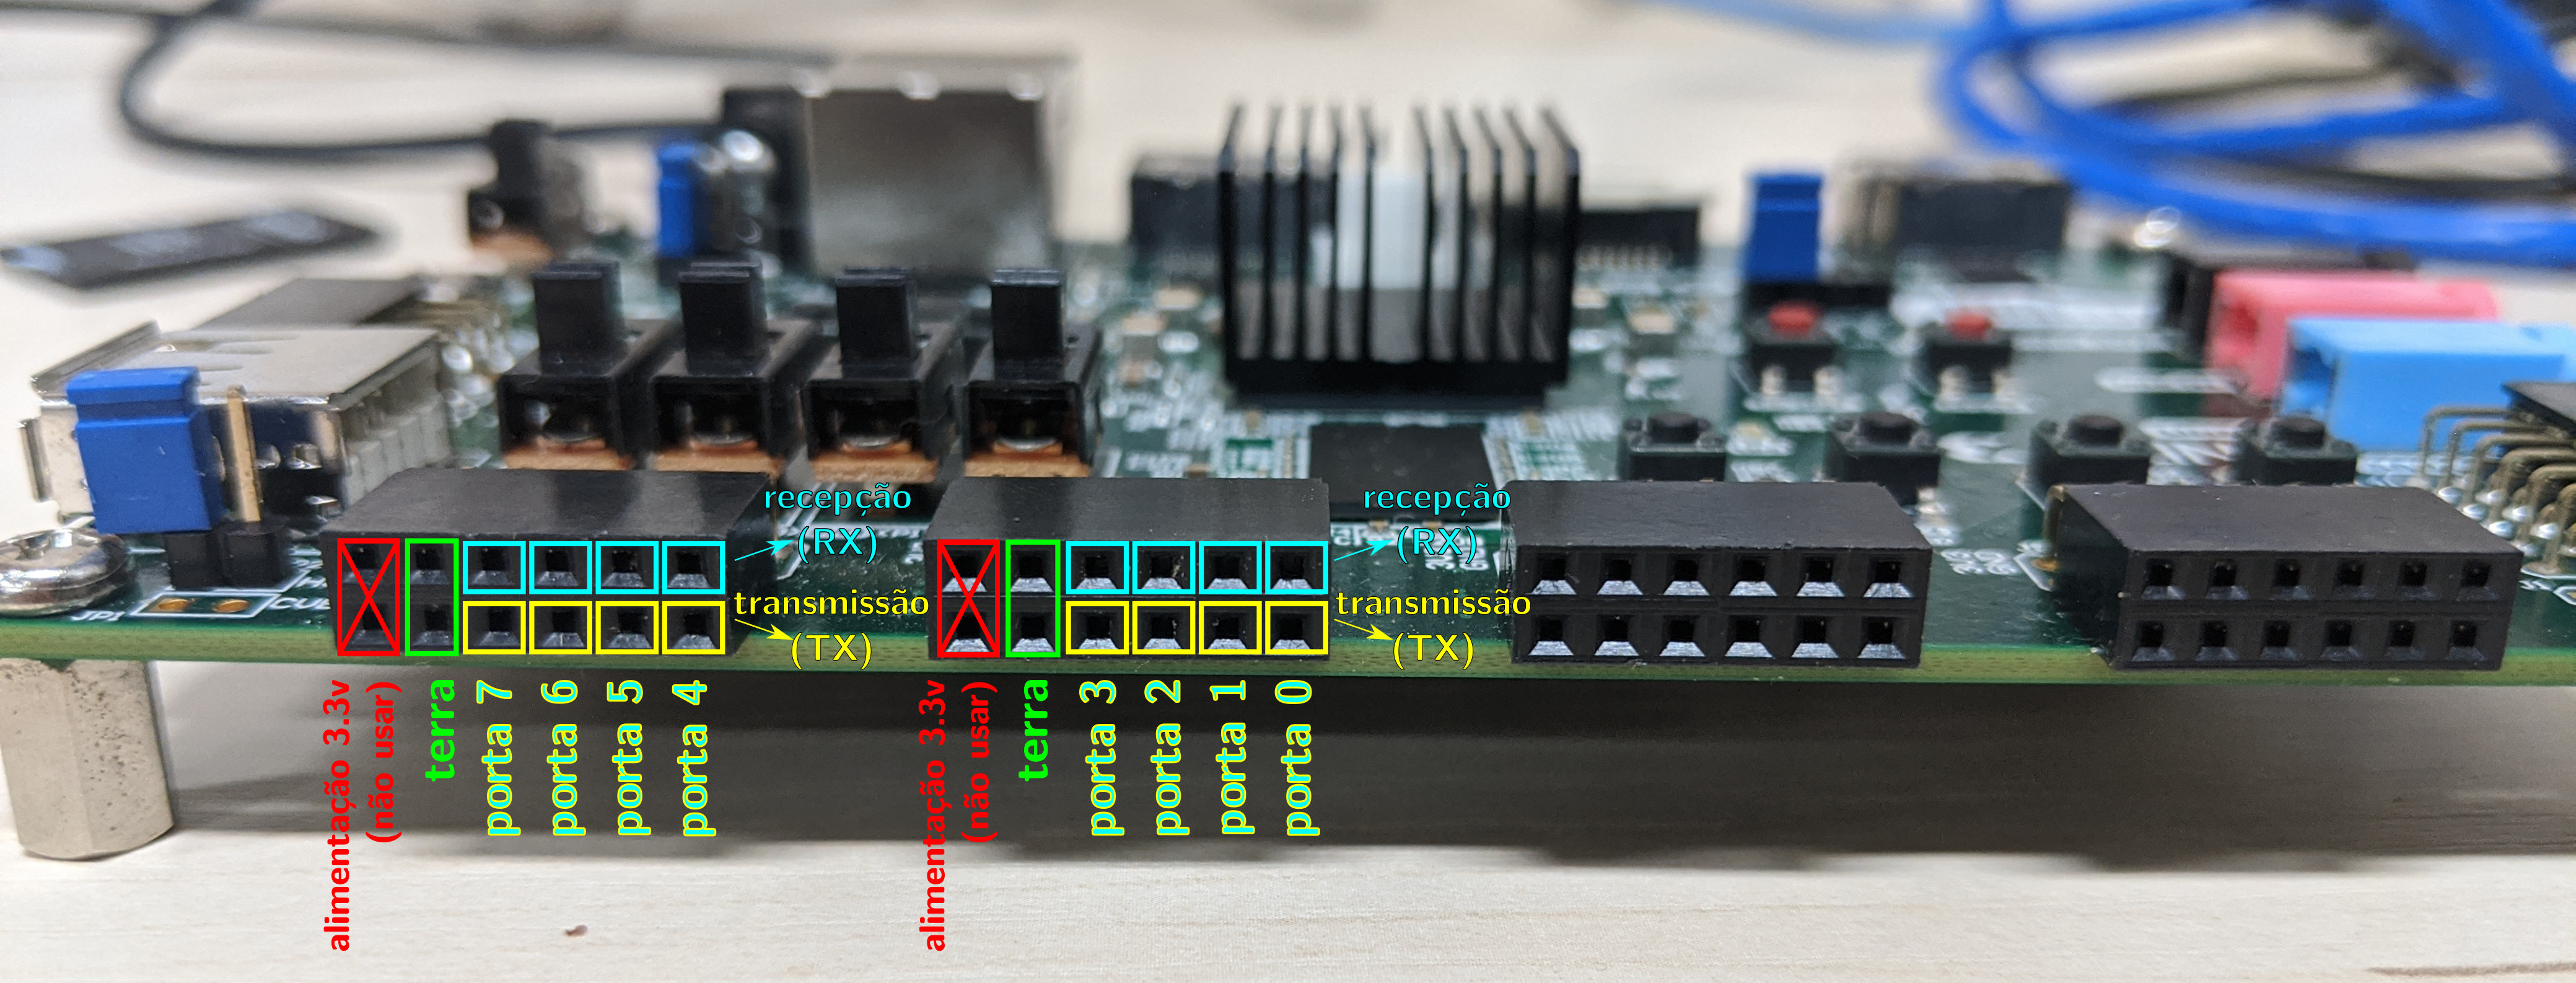
\includegraphics[width=\linewidth]{assets/portas.jpg}

    \column{0.38\linewidth}
    \eyebrow{Zybo Z7-20}
    \begin{tightitemize}
      \item FPGA expõe 8 portas seriais
      \item RX/TX/GND conectados com fios
      \item filas de TX/RX em hardware
      \item estudantes rodam a pilha Python nas placas
    \end{tightitemize}
  \end{columns}
\end{frame}

\begin{frame}[fragile]{Driver 100\% Python, sem módulo C}
  \eyebrow{UIO + mmap + descritor de arquivo}
  \begin{columns}[T,onlytextwidth]
    \column{0.59\linewidth}
\begin{lstlisting}[style=py,basicstyle=\ttfamily\tiny]
import os, mmap, fcntl, struct, asyncio

class ZyboSerialDriver:
    def __init__(self, device="/dev/uio/user_io"):
        self.fd = os.open(device, os.O_RDWR)
        fcntl.fcntl(self.fd, fcntl.F_SETFL, os.O_NONBLOCK)
        self.mm = mmap.mmap(self.fd, 0x1000)
        loop = asyncio.get_event_loop()
        loop.add_reader(self.fd, self.__irq_handler)
        self.__irq_unmask()

    def enviar(self, port, data):
        for b in data:
            offset = port * 4
            self.mm[offset:offset+4] = struct.pack("I", b)

    def __irq_handler(self):
        os.read(self.fd, 4)  # reconhece a IRQ no UIO
        elem, = struct.unpack("i", self.mm[0:4])
        port, b = elem >> 8, elem & 0xff
\end{lstlisting}

    \column{0.37\linewidth}
    \begin{tightitemize}
      \item \texttt{/dev/uio/user\_io}
      \item \texttt{mmap} dos registradores
      \item IRQ via descritor de arquivo
      \item PTY via \texttt{os.openpty()}
      \item sem extensão Python
      \item sem módulo C
    \end{tightitemize}

    \vspace{0.25em}
    {\small O kernel fornece as interfaces; o FPGA faz a temporização.}
  \end{columns}
\end{frame}

\begin{frame}{Stanford CS144: parentesco real, diferenças importantes}
  \scriptsize
  \begin{tabular}{@{}p{0.18\linewidth}p{0.36\linewidth}p{0.36\linewidth}@{}}
    \toprule
    Eixo & Stanford CS144 / Minnow & UFSCar Redes / Python\\
    \midrule
    Entrada &
    Check 0--1: \texttt{webget}, \texttt{ByteStream}, \texttt{Reassembler};
    prepara TCP por abstrações de fluxo. &
    P1: servidor IRC real; a aplicação vem primeiro para dar destino à pilha.\\
    \addlinespace[0.35em]
    TCP &
    \texttt{TCPReceiver} + \texttt{TCPSender}: seq. 32-bit, janela,
    retransmissão; interopera via TUN com TCP do Linux. &
    P2: ponta servidor sobre raw socket; handshake, ACK, FIN, timeout/RTT,
    AIMD; depois conversa com IRC.\\
    \addlinespace[0.35em]
    L3/L2 &
    Check 5: Ethernet + ARP + TAP. Check 6: roteador IP que ignora
    TCP/ARP/Ethernet. Check 7: Internet virtual sobre UDP. &
    P3: IPv4 host/roteador com LPM, TTL e ICMP Time Exceeded. P4: SLIP.
    S1: serial real em FPGA.\\
    \addlinespace[0.35em]
    Ambiente &
    C++ moderno: RAII, CMake, sanitizers, \texttt{tidy}/\texttt{format},
    testes e benchmark de desempenho. &
    Python: \texttt{bytes}, \texttt{struct}, \texttt{asyncio}, raw sockets,
    \texttt{mmap}; testes importam as camadas.\\
    \addlinespace[0.35em]
    Leitura &
    Pilha como biblioteca de sistemas, cuidadosamente fatorada em objetos. &
    Substituição incremental das camadas do Linux até uma rede física.\\
    \bottomrule
  \end{tabular}
\end{frame}

\begin{frame}{Quando Python deixa de ser a melhor escolha?}
  \eyebrow{Tecnologia de Comunicação}
  \begin{tabular}{@{}p{0.28\linewidth}p{0.28\linewidth}p{0.34\linewidth}@{}}
    \toprule
    Prática & Linguagem & Motivo principal\\
    \midrule
    Modem V.21 & C++ ou Rust & processamento em tempo real de áudio\\
    Ping E1/HDLC/ICMP & Bluespec & circuito síncrono em hardware\\
    Ethernet 10BASE-T/ARP & Bluespec & CSMA/CD completo em hardware\\
    Antenas & Python & configuração de PyNEC/OpenEMS\\
    802.11a/g offline & Python & processamento I/Q gravado\\
    \bottomrule
  \end{tabular}
\end{frame}

\begin{frame}{Modem V.21: a quebra do estilo}
  \centering
  \begin{tikzpicture}[x=1cm,y=1cm, every node/.style={font=\small}]
    \draw[very thick, caipyraLine] (0,0) -- (11,0);
    \draw[fill=caipyraRed, draw=caipyraRed] (0,0) circle (3pt);
    \node[above=0.28cm, text=caipyraRed, font=\bfseries] at (0,0) {2022};
    \node[below=0.25cm, align=center, text width=3.8cm] at (0,0) {Python: gabarito ok, alunos com underrun};
    \draw[fill=caipyraOrange, draw=caipyraOrange] (5.4,0) circle (3pt);
    \node[above=0.28cm, text=caipyraOrange, font=\bfseries] at (5.4,0) {2023};
    \node[below=0.25cm, align=center, text width=3.8cm] at (5.4,0) {C++: áudio ok, bugs de memória};
    \draw[fill=caipyraWine, draw=caipyraWine] (10.8,0) circle (3pt);
    \node[above=0.28cm, text=caipyraWine, font=\bfseries] at (10.8,0) {2024--2026};
    \node[below=0.25cm, align=center, text width=3.8cm] at (10.8,0) {C++ ou Rust};
  \end{tikzpicture}

  \vspace{1em}
  \callout{
    Aqui a taxa de processamento passa a ser parte da atividade. O risco deixa
    de ser só ``o protocolo está errado'' e vira ``o código correto não acompanha
    o tempo real''.
  }
\end{frame}

\begin{frame}{C++ ou Rust no modem}
  \begin{columns}[T,onlytextwidth]
    \column{0.58\linewidth}
    \begin{tikzpicture}
      \begin{axis}[
        width=\linewidth,
        height=5.3cm,
        ybar,
        ymin=0,
        ymax=6,
        bar width=14pt,
        symbolic x coords={2024,2025,2026},
        xtick=data,
        ylabel={grupos},
        legend style={draw=none, at={(0.5,1.02)}, anchor=south, legend columns=2},
        axis line style={caipyraLine},
        tick style={caipyraLine},
        ymajorgrids=true,
        grid style={caipyraLine},
      ]
        \addplot[fill=caipyraWine, draw=caipyraWine] coordinates {(2024,2) (2025,1) (2026,5)};
        \addplot[fill=caipyraOrange, draw=caipyraOrange] coordinates {(2024,5) (2025,5) (2026,2)};
        \legend{Rust,C++}
      \end{axis}
    \end{tikzpicture}

    \column{0.38\linewidth}
    \eyebrow{Leitura cautelosa}
    \begin{tightitemize}
      \item Rust cresceu em 2026
      \item exposição prévia formal era baixa
      \item LLMs podem reduzir o custo percebido
      \item o dado não prova causalidade
    \end{tightitemize}
  \end{columns}
\end{frame}

\begin{frame}{Por que Rust, se quase ninguém viu Rust?}
  \begin{columns}[T,onlytextwidth]
    \column{0.48\linewidth}
    \eyebrow{No recorte curricular}
    \begin{tightitemize}
      \item BCC/EnC São Carlos desde 2018: 0 planos com Rust
      \item fora do recorte: Sorocaba chegou antes, em 2023/2,
        com Tópicos Avançados em Linguagens de Programação
      \item sem pré-requisito formal (como Python em Redes em 2018)
    \end{tightitemize}

    \column{0.48\linewidth}
    \eyebrow{Motivo pragmático}
    \begin{tightitemize}
      \item menos corrupção sutil de memória
      \item erros aparecem cedo no compilador
      \item starter code pode controlar a complexidade
      \item demanda de mercado ajuda a justificar
    \end{tightitemize}
  \end{columns}
\end{frame}

\begin{frame}{Por que não ficar sempre no ecossistema Python?}
  \begin{columns}[T,onlytextwidth]
    \column{0.48\linewidth}
    \eyebrow{Alternativas possíveis}
    \begin{tightitemize}
      \item Numba para kernels numéricos
      \item Cython para extensões compiladas
      \item MyHDL e Amaranth para gerar hardware
      \item PyPy para acelerar Python puro
    \end{tightitemize}

    \column{0.48\linewidth}
    \eyebrow{Critério didático}
    \begin{tightitemize}
      \item starter code precisa ser pequeno
      \item erros precisam ser claros para iniciantes
      \item integração não pode virar o centro da prática
      \item às vezes uma linguagem dedicada tem ecossistema mais limpo
    \end{tightitemize}
  \end{columns}
\end{frame}

\begin{frame}{Por que Bluespec em E1 e Ethernet?}
  \begin{columns}[T,onlytextwidth]
    \column{0.48\linewidth}
    \eyebrow{Filosofia}
    \begin{tightitemize}
      \item capturar erros em tempo de compilação
      \item linguagem cuja semântica representa circuitos síncronos
      \item alto nível sem esconder o hardware
    \end{tightitemize}

    \column{0.48\linewidth}
    \eyebrow{Comparação com Python}
    \begin{tightitemize}
      \item MyHDL/Amaranth são ótimos geradores
      \item mas funcionam como bibliotecas Python
      \item para iniciantes, a semântica da linguagem importa
    \end{tightitemize}
  \end{columns}
\end{frame}

\begin{frame}{Onde Python continua perfeito em Telecom}
  \begin{columns}[T,onlytextwidth]
    \column{0.48\linewidth}
    \eyebrow{Simulação de antenas}
    \begin{tightitemize}
      \item Python configura PyNEC/OpenEMS
      \item bibliotecas numéricas fazem o trabalho pesado
      \item ótimo papel de linguagem de orquestração
    \end{tightitemize}

    \column{0.48\linewidth}
    \eyebrow{Wi-Fi 802.11a/g offline}
    \begin{tightitemize}
      \item transceptor com NumPy/SciPy
      \item gravação I/Q de SDR
      \item processamento fora do tempo real
      \item testes precisam rodar em tempo razoável
      \item gargalo atual: Viterbi
    \end{tightitemize}
  \end{columns}
\end{frame}

\begin{frame}{Viterbi: benchmark do gargalo}
  \begin{columns}[T,onlytextwidth]
    \column{0.58\linewidth}
    \begin{tikzpicture}
      \begin{axis}[
        width=0.88\linewidth,
        height=5.6cm,
        xbar,
        xmin=0,
        xmax=2200000,
        symbolic y coords={CPython,CPython JIT,PyPy,PyPI hard,Numba},
        ytick=data,
        xlabel={bits/s},
        scaled x ticks=false,
        xtick={0,1000000,2000000},
        xticklabels={0,1M,2M},
        xticklabel style={/pgf/number format/fixed,/pgf/number format/precision=0},
        axis line style={caipyraLine},
        tick style={caipyraLine},
        xmajorgrids=true,
        grid style={caipyraLine},
      ]
        \addplot[fill=caipyraRed!80, draw=caipyraRed] coordinates {
          (39393,CPython)
          (42247,CPython JIT)
          (336990,PyPy)
          (715022,PyPI hard)
          (1736896,Numba)
        };
      \end{axis}
    \end{tikzpicture}

    \column{0.38\linewidth}
    \eyebrow{Interpretação}
    \begin{tightitemize}
      \item JIT built-in: ganho pequeno
      \item PyPy acelera o kernel puro
      \item PyPI \texttt{viterbi} é hard-decision
      \item Numba é rápido, mas muda a dificuldade
    \end{tightitemize}
  \end{columns}
\end{frame}

\begin{frame}{JIT experimental do Python 3.14}
  \newcommand{\jitok}{\raisebox{0.25ex}{\color{caipyraRed}$\checkmark$}}
  \newcommand{\jitno}{\raisebox{0.25ex}{\color{caipyraMuted}$\times$}}
  \footnotesize
  \begin{tabular}{@{}p{0.24\linewidth}p{0.13\linewidth}>{\centering\arraybackslash}p{0.08\linewidth}p{0.45\linewidth}@{}}
    \toprule
    Distro & Pacote & JIT & comentário\\
    \midrule
    Arch Linux & python & \jitno & JIT exige clang 19; Arch usa clang 22.1.6, e clang19 está só no AUR\\
    Debian trixie & python3 & \jitno & Python 3.13; sem \texttt{sys.\_jit}\\
    Debian forky & python3.14 & \jitok & testing\\
    Fedora 44 & python & \jitok & disponível\\
    Ubuntu 26.04 LTS & python3 & \jitok & disponível\\
    Nix unstable & python314 & \jitno & nixpkgs \#331764\\
    OpenSUSE Tumbleweed & python314 & \jitok & disponível\\
    \bottomrule
  \end{tabular}

  \vspace{0.7em}
  \normalsize
  \callout{
    Para a prática, o JIT é uma curiosidade operacional, não uma estratégia de
    desempenho: no benchmark isolado, o ganho foi cerca de 4\%.
  }
\end{frame}

\begin{frame}{LLMs nas práticas de Redes}
  \begin{columns}[T,onlytextwidth]
    \column{0.58\linewidth}
    \begin{tikzpicture}
      \begin{axis}[
        width=\linewidth,
        height=5.4cm,
        ybar,
        ymin=0,
        ymax=55,
        bar width=18pt,
        symbolic x coords={2024/2,2025/1,2025/2,2026/1},
        xtick=data,
        ylabel={\% com indícios visíveis},
        nodes near coords,
        nodes near coords style={font=\scriptsize},
        axis line style={caipyraLine},
        tick style={caipyraLine},
        ymajorgrids=true,
        grid style={caipyraLine},
      ]
        \addplot[fill=caipyraRed, draw=caipyraRed] coordinates {
          (2024/2,0.0)
          (2025/1,10.3)
          (2025/2,46.2)
          (2026/1,40.0)
        };
      \end{axis}
    \end{tikzpicture}

    \column{0.38\linewidth}
    \eyebrow{Cautela metodológica}
    \begin{tightitemize}
      \item uso de LLM era permitido
      \item não é autoria comprovada
      \item são vestígios visíveis em repositórios
      \item salto claro em 2025/2
    \end{tightitemize}
  \end{columns}
\end{frame}

\begin{frame}{O que mudou em 2025}
  \centering
  \begin{tikzpicture}[x=0.92cm,y=1cm, every node/.style={font=\small}]
    \draw[very thick, caipyraLine] (0,0) -- (11.2,0);
    \draw[fill=caipyraMuted, draw=caipyraMuted] (0,0) circle (3pt);
    \node[above=0.28cm, text=caipyraMuted, font=\bfseries, align=center] at (0,0) {2022};
    \node[below=0.25cm, align=center, text width=3.0cm] at (0,0) {Copilot como autocomplete};
    \draw[fill=caipyraOrange, draw=caipyraOrange] (3.7,0) circle (3pt);
    \node[above=0.28cm, text=caipyraOrange, font=\bfseries, align=center] at (3.7,0) {fev. 2025};
    \node[below=0.25cm, align=center, text width=3.0cm] at (3.7,0) {agent mode e Claude Code previews};
    \draw[fill=caipyraRed, draw=caipyraRed] (7.4,0) circle (3pt);
    \node[above=0.28cm, text=caipyraRed, font=\bfseries, align=center] at (7.4,0) {abr.--jun. 2025};
    \node[below=0.25cm, align=center, text width=3.0cm] at (7.4,0) {Codex CLI, Codex web, Claude Code GA};
    \draw[fill=caipyraWine, draw=caipyraWine] (11.0,0) circle (3pt);
    \node[above=0.28cm, text=caipyraWine, font=\bfseries, align=center] at (11.0,0) {2025.2};
    \node[below=0.25cm, align=center, text width=2.8cm] at (11.0,0) {agentes chegam ao semestre};
  \end{tikzpicture}

  \vspace{1.1em}
  \callout{
    A ruptura não é ``IA escreve código''. A ruptura é: agentes leem o repositório,
    editam patches, rodam testes e iteram com o ambiente da prática.
  }
\end{frame}

\begin{frame}{Telecom: P1/Rust e Bluespec são leituras separadas}
  \begin{columns}[T,onlytextwidth]
    \column{0.52\linewidth}
    \eyebrow{\texttt{telecom-p1}: modem V.21}
    \footnotesize
    \begin{tabular}{@{}lrl@{}}
      \toprule
      Período & repos & indícios de LLM\\
      \midrule
      2024/1 & 7 & 0\\
      2025/1 & 6 & 2 fortes, ambos em C++\\
      2026/1 & 8 & 2 fracos, ambos em Rust\\
      \bottomrule
    \end{tabular}

    \vspace{0.55em}
    \begin{minipage}{0.9\linewidth}
      \begin{tightitemize}
        \item P1 é a única prática de Telecom com opção Rust
        \item não há causalidade comprovada entre LLMs e aumento de Rust
      \end{tightitemize}
    \end{minipage}

    \column{0.44\linewidth}
    \eyebrow{Bluespec: percepção pessoal}
    \begin{tightitemize}
      \item sem medida formal
      \item GPT-5.4 mais errava que acertava em projetos complexos
      \item GPT-5.5 mostra evolução clara
      \item por enquanto, ainda exige bastante interação humana
    \end{tightitemize}
  \end{columns}
\end{frame}

\begin{frame}{O problema filosófico}
  \Large
  Em disciplinas de final de curso, o mercado espera que estudantes saibam operar
  agentes LLM.

  \vspace{0.8em}
  \normalsize
  \callout{
    Mas se um agente consegue resolver a prática incremental quase inteira sem
    direção humana, a atividade ainda está medindo aprendizagem de Redes ou só
    execução de testes?
  }
\end{frame}

\begin{frame}{Possíveis respostas didáticas}
  \begin{tightitemize}
    \item manter testes automatizados, mas exigir defesa de decisões de protocolo
    \item avaliar depuração guiada, não só entrega que passa
    \item pedir comparação entre alternativas de implementação
    \item tornar explícito o uso de agentes e seus limites
    \item preservar práticas em que o mundo físico revela erros de integração
  \end{tightitemize}
\end{frame}

\begin{frame}{Fechamento}
  \begin{beamercolorbox}[wd=\linewidth,sep=0.55em,rounded=true]{block body}
    {\color{caipyraRed}\bfseries Python em Redes}\quad
    bom ajuste para implementar protocolos testáveis.
  \end{beamercolorbox}

  \vspace{0.55em}
  \begin{beamercolorbox}[wd=\linewidth,sep=0.55em,rounded=true]{block body}
    {\color{caipyraOrange}\bfseries C++, Rust e Bluespec em Telecom}\quad
    tempo real e hardware mudam o critério.
  \end{beamercolorbox}

  \vspace{0.55em}
  \begin{beamercolorbox}[wd=\linewidth,sep=0.55em,rounded=true]{block body}
    {\color{caipyraWine}\bfseries Agentes LLM desde 2025}\quad
    avaliação precisa medir decisão, explicação e depuração.
  \end{beamercolorbox}

  \vspace{1.5em}
  \callout{
    A pergunta central continua a mesma: que ferramenta deixa o fenômeno técnico
    mais visível para o aluno no tempo que a disciplina tem?
  }
\end{frame}

\begin{frame}{Materiais das disciplinas}
  \vspace{1.0em}
  \begin{beamercolorbox}[wd=\linewidth,sep=0.8em,rounded=true]{block body}
    {\color{caipyraRed}\bfseries Redes de Computadores}\par
    \vspace{0.2em}
    \Large\href{https://redes.matias.co.in}{\texttt{redes.matias.co.in}}
  \end{beamercolorbox}

  \vspace{0.9em}
  \begin{beamercolorbox}[wd=\linewidth,sep=0.8em,rounded=true]{block body}
    {\color{caipyraOrange}\bfseries Tecnologia de Comunicação}\par
    \vspace{0.2em}
    \Large\href{https://telecom.matias.co.in}{\texttt{telecom.matias.co.in}}
  \end{beamercolorbox}
\end{frame}

\end{document}
